\subsubsection{PSF Modeling}

Two different PSF models are currently used in the DM pipeline: PSFEx, which provides a fast preliminary PSF estimation, and Piff, used later in the pipeline for more accurate PSF modeling. During the initial data collection with \ComCam and AOS testing, most in-focus star shapes exhibited doughnut-like patterns, reflecting residual optical aberrations that had not yet been corrected. This specific form of asymmetry posed challenges for PSF modeling and was not typical. Interestingly, Piff, despite being the more advanced model, struggled to handle the large, non-symmetric PSFs compared to PSFEx. \figRef{growth_plot} shows how we were able early in the observation to constrain the PSF.


\begin{figure*}
        \centering
        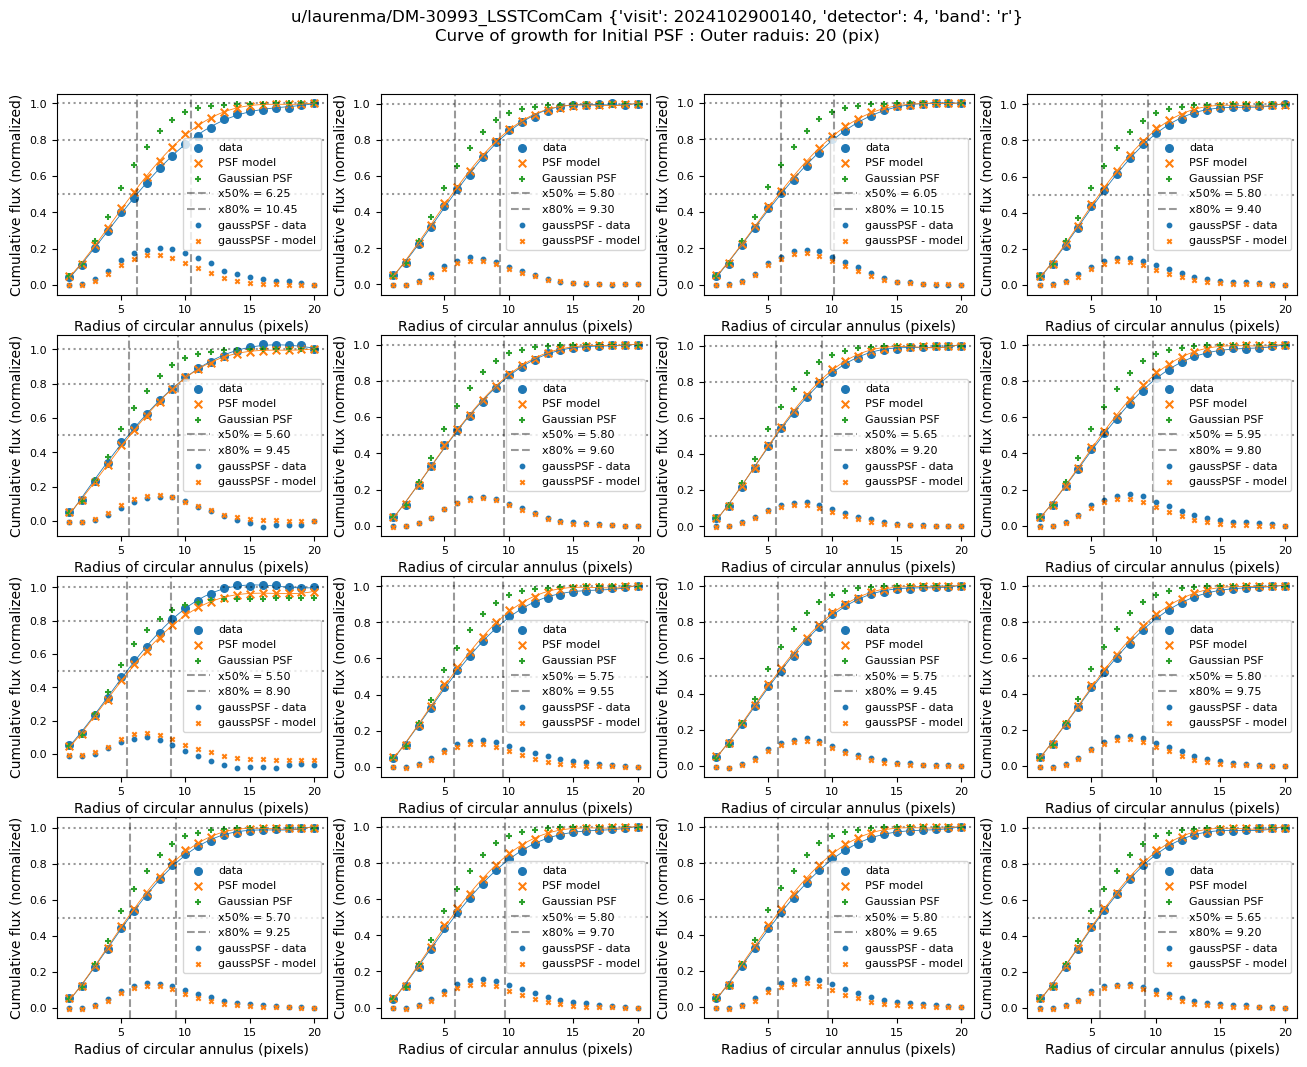
\includegraphics[scale=0.2]{figures/curveOfGrowth_pfsex_u_laurenma_DM-30993_LSSTComCam_2024102900140_4}
        \caption{\small Growth curves of the PSF compared to its model (PSFex here)  in the early data taken with \ComCam. }
        \label{fig:growth_plot}
\end{figure*}



However, as the AOS system improved image quality and produced more symmetric PSFs, we observed behavior more consistent with expectations for both PSFEx and Piff. 
Analysis of second-moment reconstructions shows that PSFEx has a systematic offset in size reconstruction
compared to Piff, which aligns with observations from DES. Overall, Piff demonstrates better PSF
reconstruction, as illustrated in \figRef{DT_plot}. \textit{Note added in proof: further analysis shows
  that Piff's relatively poor performance was due to an inconsistency between Piff's handling of the centroid
  and the convention employed by the Rubin pipelines, and that in fact Piff is able to outperform PSFEx
  on these data.}

\begin{figure*}
        \centering
        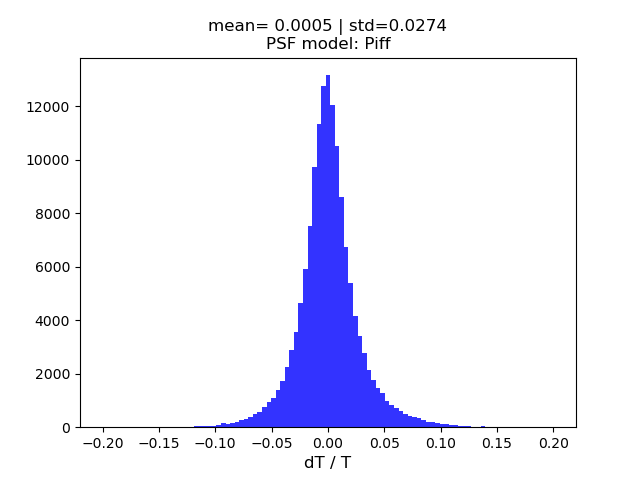
\includegraphics[scale=0.47]{figures/0_dT_1d_Piff}
        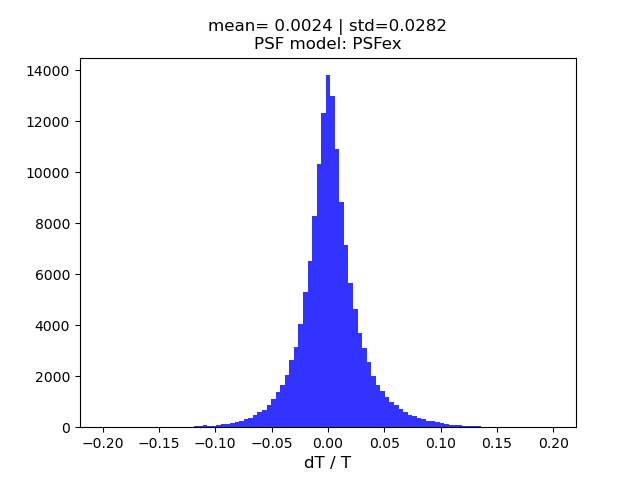
\includegraphics[scale=0.47]{figures//0_dT_1d_PSFex}
        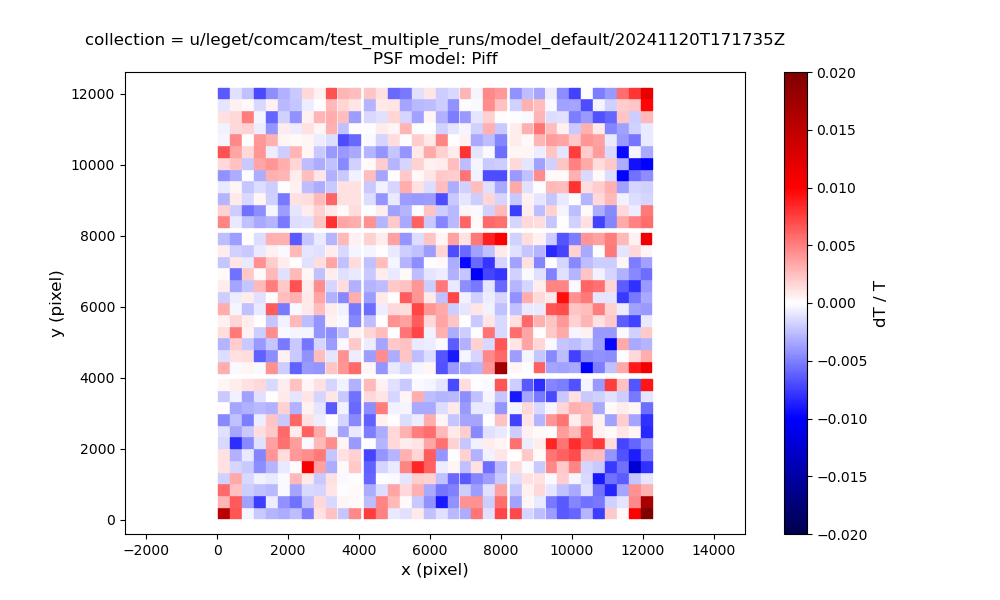
\includegraphics[scale=0.3]{figures/0_dT_2d_Piff}
	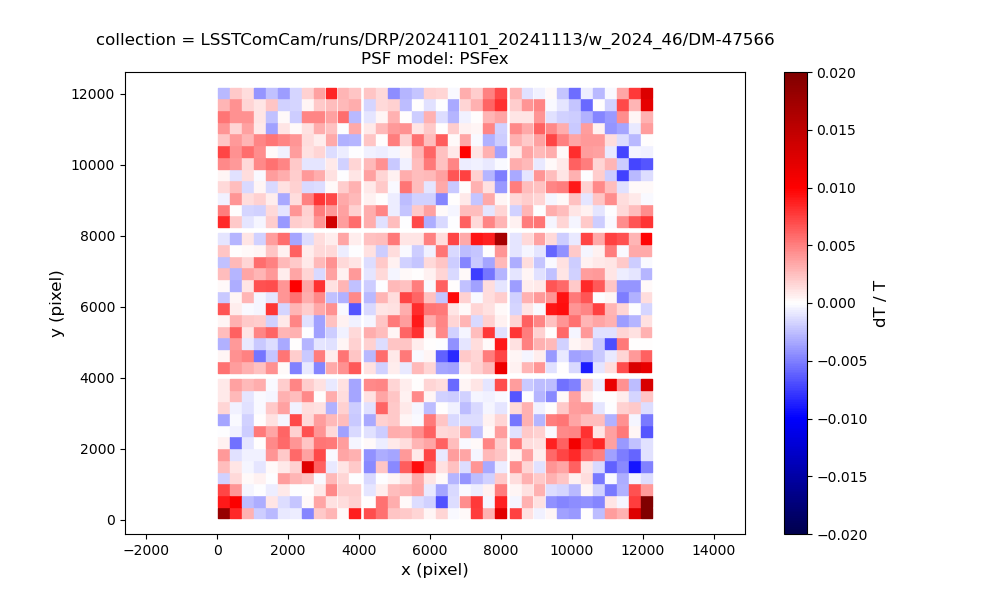
\includegraphics[scale=0.3]{figures/0_dT_2d_PSFex}
        \caption{\small Size residuals for Piff and PSFex (1d distribution and 2d average across visits). Piff has no offset and smaller scatter. Both panels 
        exhibit spatial structure across the focal plane, based on spatial averages across all science visits. The PSF is modeled per CCD in pixel coordinates 
        using a second-order polynomial for interpolation. The observed structure is unlikely to result from atmospheric or dome effects, given that this plot 
        represents an average across visits. Instead, it likely reflects spatial variations not captured by the second-order polynomial interpolation, such as 
        optical aberrations or sensor anomalies.}
        \label{fig:DT_plot}
\end{figure*}


\subsubsubsection{Understanding PSF Physics}


With LSSTCam, we aim to leverage wavefront sensor data to estimate the optical system's current state and model the optical contribution to the PSF, ultimately building a physical PSF model. During AOS testing with ComCam, the optical state was estimated using out-of-focus images to predict the optical contribution to PSF shape. A ray-tracing analysis showed that the optics fitted from these images could predict the PSF shape, providing strong evidence that a physical PSF model could be developed for LSSTCam (See \figRef{PSF_plot})


\begin{figure*}
        \centering
        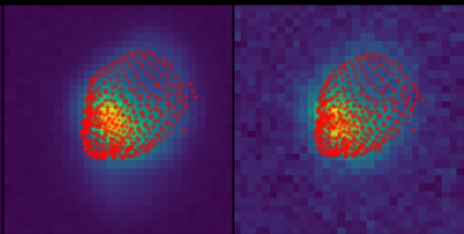
\includegraphics[scale=0.47]{figures/plot_psf_1}
        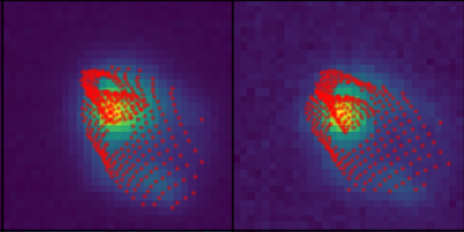
\includegraphics[scale=0.47]{figures/plot_psf_2}
        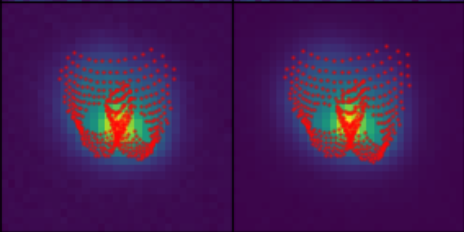
\includegraphics[scale=0.47]{figures/plot_psf_3}
        \caption{\small In-focus stars and prediction from the ray tracing on predicting PSF shape (red-dot). Optics parameters on the ray tracing side were derived from out of focus images by measuring optical aberration on "donuts" (out of focus star).}
        \label{fig:PSF_plot}
\end{figure*}